\documentclass{ctexart}
\usepackage{PhysicalChemistryNote}

\begin{document}\pagestyle{plain}
\noindent\tbf{\LARGE 2A 热力学的基本概念\footnote{本节的前两部分内容偏经验化和理论化,也没有严格的论证以支撑,在逻辑上可能也有不周之处,敬请谅解.}}\vspace{15pt}\\
\indent 热力学(Thermodynamics,源自古希腊语$\theta\ep\rho\mu o\varsigma$和$\delta\upsilon\nu\alpha\mu\iota\varsigma$),是研究热现象中物态转变和能量转换规律的学科.%
它着重研究物质的平衡状态以及与准平衡态的物理和化学过程.广义地说,热力学是研究系统宏观性质变化和系统状态变化的科学,它回答了一个过程能否发生的问题.\vspace{12pt}\\
\Section{2A.1 系统}
\Part{系统是热力学研究的对象}
\indent 我们进行科学研究时,需要确定所研究的对象,把研究的物质与其余分开(这一分隔可以是实际存在的,也可以是你假想的).我们对研究对象做如下定义.
\begin{definition}[2A.1.1 系统与环境]
    \tbf{系统}是人为划定的研究对象(以前也称为\tbf{体系}),而在系统外与系统密切相关且影响所能及的部分则称为\tbf{环境}\footnotemark.
\end{definition}
\footnotetext{你也可以简单地理解为除系统之外的其余部分.}
系统可以是一个反应容器,一台发动机,你的一个细胞,一杯水……你可以发现,系统和环境之间有时候是完全隔离的,有时候则不是.%
根据系统与环境之间的关系,我们可以对系统进行如下分类.
\begin{definition}[2A.1.2 系统的分类]
    根据系统与环境之间的关系,我们可以把系统分成如下三类.
    \begin{enumerate}[label=\tbf{\arabic*.}]
        \item \tbf{隔离系统}:系统完全不受环境的影响,和环境没有物质或能量的交换;又称为\tbf{孤立系统}.
        \item \tbf{封闭系统}:系统与环境没有物质交换,但可以有能量交换.
        \item \tbf{敞开系统}:系统与环境既可以有能量交换又可以有物质交换.
    \end{enumerate}
\end{definition}
敞开系统在我们的研究中提到的较少,而隔离系统和封闭系统是我们重点关注的研究对象.\vspace{4pt}\\
\Part{过程,途径和平衡态}
\indent 世界是变化的,系统也是变化的.
\begin{definition}[2A.1.3 过程与途径]
    给定系统的两个状态,记为始态和终态.在一定环境条件下,系统发生由始态到终态的变化,则称系统发生了一个\tbf{热力学过程},简称\tbf{过程(process)}.\\
    系统从始态到终态的变化可以由一个或者多个步骤进行,这些步骤被称作\tbf{途径(path)}.
\end{definition}
按照始态,终态的性质和过程中环境的性质,可以将过程大致分为如下几类.
\begin{definition}[2A.1.4 常见的过程]
    常见的过程有如下几类.
    \begin{enumerate}[label=\tbf{\arabic*.}]
        \item \tbf{等温过程}:系统在过程中保持温度不变,且等于恒定的环境温度.
        \item \tbf{等压过程}:系统在过程中保持压力不变,且等于恒定的环境压力.
        \item \tbf{等容过程}:系统在过程中保持的体积不变.\\
            刚性密闭容器内发生的过程一般都是等容过程.
        \item \tbf{绝热过程}:系统在过程中与环境没有热的交换,或因变化太快而来不及与环境热交换.\\
            带绝热壁的容器内的过程,或者爆炸过程,都可以视作\tbf{绝热过程}.
    \end{enumerate}
\end{definition}
一般来说,经过足够长的时间,系统总会达到一个稳定的状态,这一稳定状态下我们才能描述系统的各项性质(否则它们总是处于不断的变动中).因此,我们需要定义\tbf{平衡态}.
\begin{definition}[2A.1.5 热力学平衡状态]
    当系统的所有性质都不随时间而改变时,称系统处于\tbf{热力学平衡状态}.此时的系统须满足如下条件.
    \begin{enumerate}[label=\tbf{\arabic*.}]
        \item \tbf{热平衡}:系统各部分的温度相等.
        \item \tbf{力平衡}:系统各部分没有不平衡的力存在.
        \item \tbf{相平衡}:当系统有多个相时,物质在各相之间的分布达到平衡,相间没有物质的净转移.
        \item \tbf{化学平衡}:如果系统内各物质发生化学反应,那么达到平衡后系统的物质组成不随时间而改变.
    \end{enumerate}
\end{definition}
在本章(乃至热力学这一整个部分)我们都主要讨论平衡态(或者近平衡态)的系统.对于非平衡态的系统,我们将在之后讨论.\vspace{4pt}\\
\Part{系统的性质}
\indent 我们通常用系统的宏观可测性质(例如体积,压力,温度,物质的量,表面张力等等)%
来描述系统的热力学状态.这些性质称为\tbf{热力学变量}.根据热力学变量的性质,我们可以将其分为两类.
\begin{definition}[2A.1.5 热力学变量的分类]
    根据是否具有加和性,可以将系统的热力学变量分为如下两类.
    \begin{enumerate}[label=\tbf{\arabic*.}]
        \item \tbf{广度性质}:又称为\tbf{容量性质},其数值与系统的规模成正比.广度性质具有加和性,即系统的某种广度性质等于这系统各部分的这种广度性质的总和.
        \item \tbf{强度性质}:其数值与系统的规模无关,不具有加和性(例如,你不能把两杯$50\tccentigrade$的水混在一起并宣称现在它们是$100\tccentigrade$的).
    \end{enumerate}
\end{definition}
常见广度性质有物质的量,质量,热力学能\footnote{我们将在\tbf{2B}中提到热力学能的概念.}等;常见强度性质有压力,温度,密度,黏度等等.\\
\indent 回顾我们在\tbf{1A.1}中提到的状态函数,是为了描述系统的状态而存在的.因此,同一个状态的系统应当对应一个固定的状态函数值,%
而不论它是由什么途径得到的.因此,我们给出状态函数的严格定义.
\begin{definition}[2A.1.6 状态函数]
    处于平衡状态的热力学系统,若其宏观物理量具有确定的值,并且这些物理量仅由系统所处的状态所决定,与达到平衡态的过程无关,我们就称这一物理量为系统的\tbf{状态函数}.
\end{definition}\vspace{8pt}
\Section{2A.2 热平衡,热力学第零定律和热}
\indent 我们在\tbf{1A}中给出了温度的粗浅的定义,现在我们详细地再次论述这一概念.\\
\indent 温度的概念最初源于人类对冷热现象的直观感知.在日常生活中,人们通过触觉区分物体的“冷”与“热”,%
例如感知火焰的灼热,冰雪的寒冷,或通过观察自然现象(如水结冰或沸腾)推测环境温度的变化.%
古代文明已尝试量化冷热程度,例如中国汉代用“炭火变色”判断冶炼温度,古希腊通过混合冷热水调节沐浴温度.%
然而,这些方法依赖主观感受或经验观察,缺乏普适性和精确性.\\
\indent 17世纪后,随着温度计的发明,温度的测量逐渐脱离主观感知,成为基于物质热膨胀性质的客观物理量.%
例如,水银温度计通过液柱长度变化反映温度差异,首次将冷热程度转化为可量化,可复现的数值.这一工具的发展促使科学家追问温度的本质,%
最终通过热力学与统计力学的理论框架,将生活中的“冷热”抽象为描述系统热运动强度的物理量——温度.\\
\indent 我们不禁要问:为什么温度计能测定温度呢?这就要从它的原理——\tbf{热平衡}开始讲起.
\begin{definition}[2A.2.1 热平衡]
    当两个或多个热力学系统通过导热壁(允许热量传递的界面)接触时,若它们的宏观性质在长时间后不再发生任何变化,则称这些系统达到了\tbf{热平衡}.此时,系统间的净热流量为零,但微观粒子仍存在动态的能量交换.
\end{definition}
那么,温度计是如何判定温度相等的呢?换句话说,如果它和两个不同物体都建立了热平衡,这两个物体之间是否也能建立平衡呢?大量实验事实表明,热平衡具有递推性.
\begin{theorem}[2A.2.2 热力学第零定律]
    若两个热力学系统均与第三个系统处于热平衡状态,此两个系统也必互相处于热平衡.
\end{theorem}
热力学第零定律不能通过任何理论上的推导得出,这是一条类似数学中的公理的定律.\\
\indent 在我们的设想中,建立了热平衡的两个系统必定有一个相等的状态函数,我们就定义这一状态函数为\tbf{温度}.%
简而言之,如果两个系统建立了热平衡,那么它们的温度相等.%
热力学第零定律的实质是指出了温度这一状态函数的存在,并且给出了一种比较温度的方法.%
在比较各个系统的温度时,不需要将它们互相接触,只需将一个作为标准的第三系统分别于各个系统接触达到热平衡即可.%
这个作为标准的第三系统就是\tbf{温度计}.\\
\indent 人们对于热的本质的认识进行了长时间的探寻,一段时间内错误的“热质说”也甚嚣尘上.%
经由我们在\tbf{1B}中对温度的统计学概念的讨论,我们知道温度可以衡量微观分子做无规则运动的强度(实际上是平动能).%
当温度不同的系统接触时,应当通过分子的碰撞交换能量.经由这种方式交换的能量就是\tbf{热}.
\begin{definition}[2A.2.3]
    \tbf{热}是由于温度不同而在系统与环境之间交换或传递的能量,用符号$Q$表示.\\
    当系统吸热时,$Q$取正值,即$Q>0$;系统放热时,$Q$取负值,即$Q<0$.
\end{definition}
\begin{hint}
    热力学中的最基本的概念,即温度和热量,常常难以界定的十分妥帖.人们为了先有温度再有热量还是先有热量再有温度争论了许久.\\
    一种观点认为,应该先引入温度的概念,然后定义热量为两个不同温度的系统接触时传递的能量;%
    另一种观点认为,应该首先讨论热平衡(即宏观上没有热量的流动),然后定义温度为两个处于热平衡的系统所共有且相等的状态函数.%
    应当说,温度和热量是两个相互依存的物理量,它们之间在逻辑上是循环的关系.\\
    不过,你也许应当把主要的精力放在研究热力学的基本原理和将它们应用于解决化学中的实际问题,%
    而非刻意追求形式逻辑上的圆满.毕竟这不是数学,而我们的理论已经能相当好地描述这个世界了.
\end{hint}
\vspace{8pt}
\Section{2A.3 功}
\Part{功的定义}
\indent 你也许在初中物理中已经学过机械功,电功等等关于功的概念.在热力学中,功的定义如下.
\begin{definition}[2A.3.1 功]
    除了热以外以其它各种形式传递的能量称为\tbf{功},用符号$W$表示.\\
    系统对外做功时,$W$取负值,即$W<0$;环境对系统做功时,$W$取正值,即$W>0$.
\end{definition}
\begin{hint}
    有别于我们提到的各种状态函数,功和热都是依赖于途径的.%
    因此,为了以示区别,功和热对应的小量改用$\delta$表示,而非其它状态函数所用的微分符号$\di$.
\end{hint}
一般来说,各种形式的功都是广度量和强度量的乘积.%
例如机械功是位移$\di x$与力$F$的乘积,即
\[\delta W=F\di x\]
而电功是电势差$E$与电荷量$\di Q$的乘积,即
\[\delta W=E\di Q\]
等等.强度量决定了能量的传递方向,广度量决定了功的大小.\\
\indent 宏观地看,功是大量质点以有序运动而传递的能量,热是大量质点以无序运动传递的能量.\vspace{4pt}\\
\Part{膨胀功}
\indent 气体的膨胀会对外界做功,这是机械功的一种简单的体现.%
设想气体存放在带活塞(与器壁之间无摩擦)的容器中,容器横截面积为$A$.设气体压力为$p_\i$,外界压力为$p_\e$\footnote{此处的$\i$和$\e$分别指internal和external,用于表示内压和外压.}.%
当$p_\i>p_\e$时,气体就会向外膨胀,对外界做功.%
设活塞移动的距离为$\dx$,于是气体做的膨胀功$\delta W$为
\[\delta W=-F_\e\dx=-\left(\dfrac{F_\e}{A}\right)(A\dx)=-p_\e\di V\]
需要注意的是,由于气体是对环境做功,因此计算力$F$时应当计算外界对活塞的压力(你可以想象活塞上放了一个重物,重物对活塞的压力为$F_\e$,那么气体膨胀的力将用于抬升该重物,该力与抬升距离的乘积就是气体所做的功).\\
\indent 根据膨胀过程中外压的不同,我们可以对其做如下分类.
\begin{definition}[2A.3.2]
    我们大致将气体的膨胀分为如下几类.
    \begin{enumerate}[label=\tbf{\arabic*.}]
        \item \tbf{自由膨胀}:外压$p_\e$恒为$0$,即气体向真空膨胀.
        \item \tbf{恒外压膨胀}:外压$p_\e$恒为一定值.
        \item \tbf{准静态膨胀}\footnotemark :外压$p_\e$保持比内压$p_\i$大一个无穷小量$\di p$.
    \end{enumerate}
\end{definition}
\footnotetext{此处的(以及本节之后的)准静态膨胀是指等温条件下的准静态膨胀.我们在\tbf{2C}中还会看到绝热条件下的准静态膨胀.}
\indent 假定我们研究的气体是理想气体.现在,我们逐一推导在上述几种过程下气体从体积$V_1$膨胀到$V_2$时所做的功.
\begin{derivation}
    \begin{enumerate}[label=\tbf{\arabic*.}]
        \item 自由膨胀时,我们有
            \[W=\int_{V_1}^{V_2}0\di V=0\]
            这表明气体自由膨胀时不对外做功.
        \item 对抗恒外压膨胀时,我们有
            \[W=\int_{V_1}^{V_2}-p_\e\di V=-p_\e\left(V_2-V_1\right)\]
            如果气体发生了多次恒外压膨胀,那么只需分别计算即可.
        \item 我们首先考虑气体体积变化为无穷小量$\di V$时,气体做的功
            \[\delta W=-p_\e\di V=-\left(p_\i+\di p\right)\di V\]
            注意到其中有一个二阶无穷小量$\di p\di V$,可以忽略(通俗地来说,你可以认为$\di p\ll p_\i$,因此可以忽略不计),%
            于是积分可得
            \[W=\int_{V_1}^{V_2}-p_\i\di V=\int_{V_1}^{V_2}-\dfrac{nRT}{V}\di V=-nRT\ln\dfrac{V_2}{V_1}\]

    \end{enumerate}
\end{derivation}
如果我们观察$p-V$图像,就可以发现准静态膨胀是同一过程下系统做功最大的途径.\\
当我们将$p-V$曲线下的矩形取得足够细时,系统压力$p_\i$和环境压力$p_\e$差别足够小而可以忽略,此时众多的矩形的面积之和%
(根据定积分的定义)就等于$p-V$曲线下围的面积,也就是准静态膨胀所做的功.除此之外的任何一种膨胀方式,所做的功均小于等于该曲线下围的面积.
\begin{figure}[H]
    \centering\documentclass{standalone}
\usepackage{PhysicalChemistryNote}
\begin{document}
\begin{tikzpicture}
    \filldraw[lightgray] (0.3,0)--(0.3,1/3.3)--(3.3,1/3.3)--(3.3,0)--(0.3,0);
    \draw[->] (0,0) -- (4,0) node[right]{$V$};
    \draw[->] (0,0) -- (0,3.5) node[above]{$p$};
    \draw[domain=0.3:3.3] plot[smooth](\x,1/\x);
    \draw[dashed] (0.3,1/0.3) -- (0.3,0) node[below]{$V_1$};
    \draw[dashed] (3.3,1/3.3) -- (3.3,0) node[below]{$V_2$};
    \draw[dashed] (0.3,1/3.3) -- (3.3,1/3.3) node[right]{$p_\e$};
\end{tikzpicture}
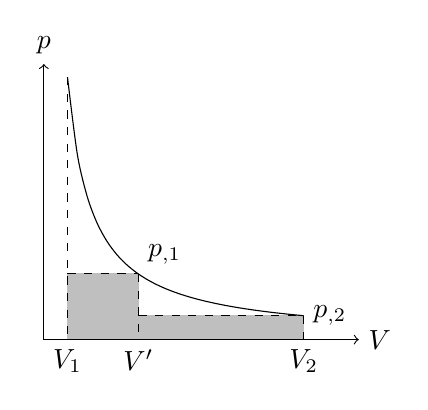
\begin{tikzpicture}
    \filldraw[lightgray] (0.3,0)--(0.3,1/1.2)--(1.2,1/1.2)--(1.2,1/3.3)--(3.3,1/3.3)--(3.3,0)--(0.3,0);
    \draw[->] (0,0) -- (4,0) node[right]{$V$};
    \draw[->] (0,0) -- (0,3.5) node[above]{$p$};
    \draw[domain=0.3:3.3] plot[smooth](\x,1/\x);
    \draw[dashed] (0.3,1/0.3) -- (0.3,0) node[below]{$V_1$};
    \draw[dashed] (3.3,1/3.3) -- (3.3,0) node[below]{$V_2$};
    \draw[dashed] (1.2,1/1.2) -- (1.2,0) node[below]{$V'$};
    \draw[dashed] (0.3,1/1.2) -- (1.2,1/1.2) node[above right]{$p_{\e,1}$};
    \draw[dashed] (1.2,1/3.3) -- (3.3,1/3.3) node[right]{$p_{\e,2}$};
\end{tikzpicture}
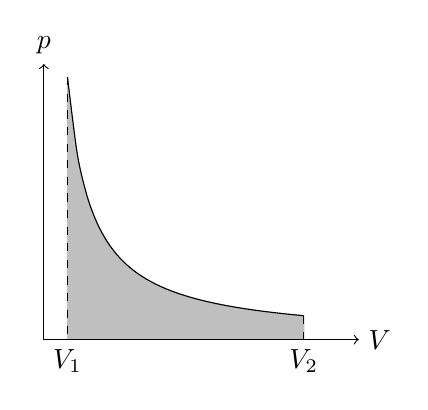
\begin{tikzpicture}
    \filldraw[lightgray] (0.3,0)--plot[domain=0.3:3.3,smooth](\x,1/\x)--(3.3,0);
    \draw[->] (0,0) -- (4,0) node[right]{$V$};
    \draw[->] (0,0) -- (0,3.5) node[above]{$p$};
    \draw[domain=0.3:3.3] plot[smooth](\x,1/\x);
    \draw[dashed] (0.3,1/0.3) -- (0.3,0) node[below]{$V_1$};
    \draw[dashed] (3.3,1/3.3) -- (3.3,0) node[below]{$V_2$};
\end{tikzpicture}
\end{document}
\end{figure}
\indent 由此可见,即使始态和终态一样,过程中做的功$W$也会随着途径的改变而改变.%
因此,功不是状态函数,它与变化的途径有着密切的联系.同样地,热也具有这样的性质.%
我们不能说系统中含有多少功或热,只能在具体的变化过程中求出功和热.\vspace{4pt}\\
\Part{压缩功}
\indent 与膨胀功类似,当气体被压缩时,环境对气体做功.我们来看以下三种对气体做功的方式.
\begin{figure}[H]
    \centering\documentclass{standalone}
\usepackage{PhysicalChemistryNote}
\begin{document}
\begin{tikzpicture}
    \filldraw[lightgray] (0.3,0)--(0.3,1/0.3)--(3.3,1/0.3)--(3.3,0)--(0.3,0);
    \draw[->] (0,0) -- (4,0) node[right]{$V$};
    \draw[->] (0,0) -- (0,3.5) node[above]{$p$};
    \draw[domain=0.3:3.3] plot[smooth](\x,1/\x);
    \draw[dashed] (0.3,1/0.3) -- (0.3,0) node[below]{$V_1$};
    \draw[dashed] (3.3,1/0.3) -- (3.3,0) node[below]{$V_2$};
    \draw[dashed] (0.3,1/0.3) -- (3.3,1/0.3) node[right]{$p_\e$};
\end{tikzpicture}
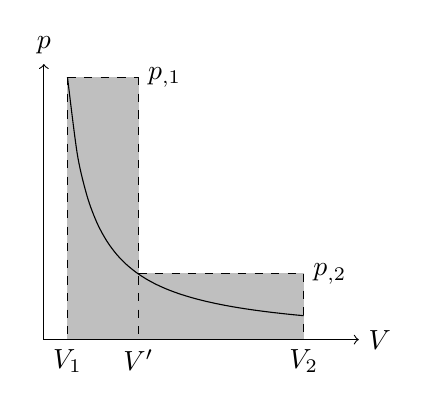
\begin{tikzpicture}
    \filldraw[lightgray] (0.3,0)--(0.3,1/0.3)--(1.2,1/0.3)--(1.2,1/1.2)--(3.3,1/1.2)--(3.3,0)--(0.3,0);
    \draw[->] (0,0) -- (4,0) node[right]{$V$};
    \draw[->] (0,0) -- (0,3.5) node[above]{$p$};
    \draw[domain=0.3:3.3] plot[smooth](\x,1/\x);
    \draw[dashed] (0.3,1/0.3) -- (0.3,0) node[below]{$V_1$};
    \draw[dashed] (3.3,1/1.2) -- (3.3,0) node[below]{$V_2$};
    \draw[dashed] (1.2,1/0.3) -- (1.2,0) node[below]{$V'$};
    \draw[dashed] (0.3,1/0.3) -- (1.2,1/0.3) node[right]{$p_{\e,1}$};
    \draw[dashed] (1.2,1/1.2) -- (3.3,1/1.2) node[right]{$p_{\e,2}$};
\end{tikzpicture}
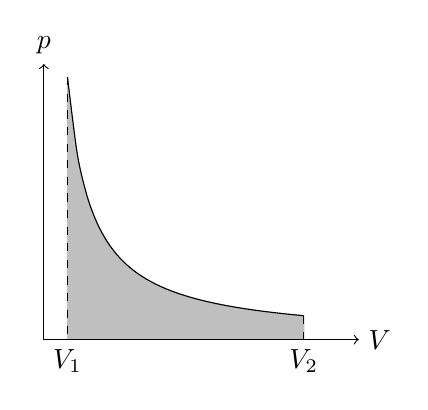
\begin{tikzpicture}
    \filldraw[lightgray] (0.3,0)--plot[domain=0.3:3.3,smooth](\x,1/\x)--(3.3,0);
    \draw[->] (0,0) -- (4,0) node[right]{$V$};
    \draw[->] (0,0) -- (0,3.5) node[above]{$p$};
    \draw[domain=0.3:3.3] plot[smooth](\x,1/\x);
    \draw[dashed] (0.3,1/0.3) -- (0.3,0) node[below]{$V_1$};
    \draw[dashed] (3.3,1/3.3) -- (3.3,0) node[below]{$V_2$};
\end{tikzpicture}
\end{document}
\end{figure}
可以发现,准静态压缩所做的功是最小的,而一次性恒外压压缩所做的功是最大的.\vspace{12pt}\\
\Section{2A.4 准静态过程和可逆过程}
\Part{准静态过程}
\indent 我们已经在\tbf{2A.3.2}中提到了准静态膨胀.现在,我们对准静态过程进行较为严谨的定义.
\begin{definition}[2A.4.1 准静态过程]
    如果在一个过程的每个瞬间,系统都接近于平衡状态,其状态函数在系统的各部分都有确定的取值,整个系统可以看成一系列极接近平衡的状态构成,这样的过程被称作\tbf{准静态过程}.
\end{definition}
在准静态膨胀中,不论何时内外压仅相差一个无穷小量$\di p$,可以近似地看作内外力平衡,因而是准静态过程.\\
\indent 准静态过程在实际上是办不到的(你不可能让一个系统在变化的同时时刻保持平衡),但当一个过程进行地很慢时,这个过程就趋近于准静态过程.\vspace{4pt}\\
\Part{可逆过程}
\indent 考虑我们在上面提到的准静态膨胀和准静态压缩过程,你可以发现膨胀时系统对环境做的功恰好等于压缩时环境对系统做的功.%
换句话说,如果你把膨胀时做的功收集起来(例如转化为重力势能)并再次压缩,那么系统将复原.\\
\indent 然而,如果你采取了其它的膨胀方式,就会发现无论如何你不能用膨胀所做的功再将其压缩回原来的状态.%
如果你执意这么做,就会发现环境发生了不可逆的变化:它向系统做功,自己得到热\footnote{关于功和热转化的不可逆性,我们将在\tbf{Chapter 3}中讨论.}.\\
\indent 显然,准静态膨胀和压缩是特殊的,经过准静态膨胀后可以在不造成任何影响的情况下将系统和环境复原.这是一种在热力学中极为重要的过程,即\tbf{可逆过程}.
\begin{definition}[2A.4.2 可逆过程]
    \tbf{可逆过程}是指过程发生后能够被复原并对系统本身或外界不产生任何影响的过程;%
    另一种定义是系统能够在无能量损失或耗散的情形下通过无穷小的变化实现反转的热力学过程.\\
    反之,如果采取任何方法都不能使系统和环境复原,就称为\tbf{不可逆过程}.\\
    如果这一过程是一个循环的过程,那么系统和环境将恢复初始态而没有任何变化,称这样的过程为\tbf{可逆循环}.
\end{definition}
很多实际过程都可以视作可逆过程,例如液体在沸点的蒸发,可逆电池在外加电动势和电池电动势近似相等时的充电和放电,等等.\\
\indent 以后我们将会知道,可逆过程是能量利用效率最高的过程.
\end{document}